\documentclass[11pt,a4paper]{article}
\usepackage[utf8]{inputenc}
\usepackage[english]{babel}
\usepackage[margin=2cm]{geometry}
\usepackage{amsmath,amssymb,amsfonts}
\usepackage{graphicx}
\usepackage{xcolor}
\usepackage{hyperref}
\usepackage{booktabs}
\usepackage{array}
\usepackage{ragged2e}
\usepackage{float}
\usepackage{listings}
\usepackage{tikz}
\usetikzlibrary{shapes,arrows,positioning,calc}

\definecolor{primarycolor}{RGB}{30, 60, 110}
\definecolor{secondarycolor}{RGB}{235, 240, 245}
\definecolor{codebackground}{RGB}{248, 248, 248}
\definecolor{commentcolor}{RGB}{100, 100, 100}
\definecolor{keywordcolor}{RGB}{170, 13, 145}
\definecolor{stringcolor}{RGB}{196, 26, 22}

\hypersetup{colorlinks=true,linkcolor=primarycolor,urlcolor=primarycolor,
pdftitle={Architecture with Dynamic Associative Memory in Transformer Models}}

\lstset{language=Python,backgroundcolor=\color{codebackground},basicstyle=\ttfamily\small,
keywordstyle=\color{keywordcolor}\bfseries,commentstyle=\color{commentcolor}\itshape,
stringstyle=\color{stringcolor},breaklines=true,showstringspaces=false,frame=single,
rulecolor=\color{black!20},tabsize=4}

\title{\textbf{\Large \color{primarycolor} Architecture with Dynamic Associative Memory in Transformer Models}}
\author{\Large \textbf{Alex Goldenstein} \\ \vspace{0.3cm} \normalsize \textbf{Status:} Comprehensive Architectural and Methodological Specification}
\date{\today}

\begin{document}
\RaggedRight
\maketitle
\hrule
\vspace{0.5cm}

\section{Introduction and Architectural Problem Statement}

The proposed Cognitive Master Architecture is a hybrid cognitive architecture combining neural processing methods (Transformer) with external structured associative memory (LTM with graph topology and offline consolidation). Rather than treating conventional language models as collections of isolated token operations, this architecture introduces a structure oriented toward continuous accumulation and integration of new experience and knowledge. Previously acquired knowledge is used in subsequent communication, enabling progressively better results. The unit of communication is a dialogue, technically accumulating the context of a session.

\subsection*{Dialogue ($\mathcal{D}$)}
\textbf{Dialogue} $\mathcal{D}=\{T_1,T_2,\dots,T_N\}$ is formalized as a single dynamic process and an integral unit of discussion. Each turn $T_n$ produces semantic activity that accumulates in the dialogue graph $G_{\mathcal{D}}$, recording transitions between topics and user intentions.

\subsection*{D-Context ($\mathbf{s}_{\mathcal{D}}$)}
\textbf{D-Context} is the state of the current dialogue maintained inside the associative-memory module. It aggregates the semantic core of the discussion---topic, intentions, and contextual constraints---into the integrated state $\mathbf{s}_{\mathcal{D}}$. D-Context is created when a new dialogue starts. The first message $T_1$ initializes and anchors it; full memory information conditioned on D-Context begins to flow back into the Transformer from the second message $T_2$ onward.

The classical Transformer architecture exhibits a strict dichotomy between static parametric memory in the weight matrices ($W_Q,W_K,W_V,W_O,W_{\text{mlp}}$) and the dynamic but strictly length-limited Attention Context Window.

Adapting to new domains, tasks, or real-world facts requires either resource-intensive parametric adaptation (Fine-Tuning / PEFT), with the risk of catastrophic forgetting, or loading large datasets into the prompt (In-Context Learning / RAG), producing quadratic computational growth $\mathcal{O}(N^2)$ and noise.

\subsection*{Goal and Conceptual Solution}
Construct a \textbf{hybrid multi-level semantic-associative memory system} functioning as an internal--external Transformer module:
\begin{enumerate}
\item \textbf{Level I (Base Invariant):} Extract and fix (``freeze'') a universal asemantic geometric basis of the hidden activation space, $\mathcal{B}\subset\mathbb{R}^d$, once for the entire model.
\item \textbf{Level II (Dynamic Semantic Graph):} For a specific downstream task $T$, automatically prune irrelevant basis elements and impose directed causal and co-activation edges, forming the directed semantic graph $G_T$.
\item \textbf{Level III (OOD Induction):} As the external world changes, detect residual energy in activation space and inductively create new graph nodes and edges in real time without retraining the base neural network (Zero Re-Training / Continual Learning).
\end{enumerate}

\section{Closed-Loop Interaction between the Transformer and Associative Memory}

Constructing the dictionary and semantic graph defines the structure of memory, but using that memory requires an explicit return path from memory to the Transformer. In the proposed architecture this path is implemented directly in the Transformer's internal hidden-state space.

\subsection*{Two-Phase Target-Layer Interface}

Memory communication uses a target layer $l_{\text{target}}$ of the selected Transformer model. The selected layer is simply doubled: the original part becomes the source for update, while the new part becomes the interface into which associative memory inserts its messages. This creates two logical directions of communication:
\begin{enumerate}
\item \textbf{Read Phase (Input Pole):} at the input to $l_{\text{target}}$, the current hidden state $h_t^{(l_{\text{target}}^{\text{in}})}$ is captured. It is used as a query to associative memory and to update D-Context without interrupting the Transformer's main computational stream.
\item \textbf{Return and Reintegration Phase (Output Pole):} associative memory uses the query, D-Context, and active structure $G_T$ to form the latent memory vector $\Delta h_t$. It is returned to the Transformer at the output of the target layer and integrated into the Residual Stream:
\begin{equation}
\tilde h_t^{(l_{\text{target}}^{\text{out}})}=h_t^{(l_{\text{target}}^{\text{out}})}+\Delta h_t^{(\mathcal D)}.
\end{equation}
\end{enumerate}

The resulting closed loop is
\[
\text{Transformer hidden state}\rightarrow\text{Associative Memory}\rightarrow
\text{D-Context / }G_T\rightarrow\Delta h_t\rightarrow\text{Transformer}.
\]

Introducing an internal language elegantly solves the direct ``vectors $\rightarrow$ graph'' interface problem. In this interpretation the system becomes a Neuro-Symbolic AI hybrid in which the Transformer acts as the ``processor'' and the internal language as a ``system assembler'' issuing commands to memory and execution blocks.

In effect, the preceding discussion defines the language of internal communication of the cognitive system. It is fully determined by the selected Transformer and its original training. We now consider how the system's associative memory can learn this language and use it.

\subsection*{How the Internal Language Solves the Translation Problem}
\begin{enumerate}
\item \textbf{Separation of responsibility:} the Transformer no longer needs to know exactly how the graph is organized in the database. Its task is to reason and express intent in a strictly deterministic machine-readable language (symbolic protocol).
\end{enumerate}

The system's internal language is the Transformer's own internal language. It is read from an optimally selected internal layer. Associative memory knows nothing except this language: it learns it from scratch, first building activation patterns and then, on their basis, sequences and temporal relationships.

This conceptual shift changes the architecture completely, turning it from a neuro-symbolic hybrid into a purely endogenous neuro-associative system.

If the internal language consists of vector activations of one internal Transformer layer (Internal Latent Representation), while associative memory is initially ``blind'' to human language and learns from those activations from scratch, the system operates directly in the Transformer's internal representation space.

\subsubsection*{Architectural View}
\begin{figure}[H]
\centering
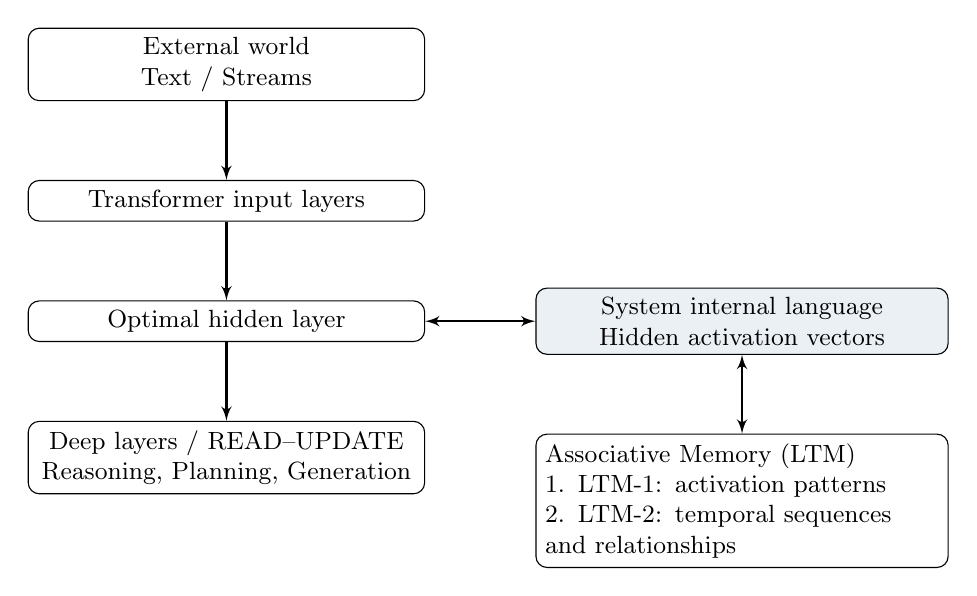
\begin{tikzpicture}[node distance=1.0cm and 1.2cm, >=latex', every node/.style={font=\small}]
\node[draw,rounded corners,align=center,text width=4.8cm](world){External world\\Text / Streams};
\node[draw,rounded corners,below=of world,align=center,text width=4.8cm](input){Transformer input layers};
\node[draw,rounded corners,below=of input,align=center,text width=4.8cm](hidden){Optimal hidden layer};
\node[draw,rounded corners,right=1.4cm of hidden,align=center,text width=5.0cm,fill=secondarycolor](lang){System internal language\\Hidden activation vectors};
\node[draw,rounded corners,below=of hidden,align=center,text width=4.8cm](deep){Deep layers / READ--UPDATE\\Reasoning, Planning, Generation};
\node[draw,rounded corners,below=of lang,align=left,text width=5.0cm](mem){Associative Memory (LTM)\\1. LTM-1: activation patterns\\2. LTM-2: temporal sequences and relationships};
\draw[->,thick](world)--(input); \draw[->,thick](input)--(hidden); \draw[<->,thick](hidden)--(lang);
\draw[->,thick](hidden)--(deep); \draw[<->,thick](lang)--(mem);
\end{tikzpicture}
\caption{The Transformer's endogenous internal language as the associative-memory interface.}
\end{figure}

\subsubsection*{Main Advantages of the Concept}
\begin{enumerate}
\item \textbf{Zero Translation Loss:} continuous meanings do not have to be translated into discrete JSON, Cypher, or a textual DSL. Memory operates on the native mathematical objects---vectors and tensors---used by the Transformer itself.
\item \textbf{Semantic Density and Unbiased Semantics:} the internal latent space of a deep Transformer layer contains richer semantics---context, intonation, and associations---than an individual human word.
\item \textbf{Self-Organization / Unsupervised Emergence:} LTM learns from scratch:
\begin{itemize}
\item \textbf{Stage 1 (LTM-1):} memory records frequent static activation configurations, creating the base dictionary of the system's internal atomic meanings.
\item \textbf{Stage 2 (LTM-2):} using stable LTM-1 nodes, memory learns trajectories of state change over time, $\mathrm{State}_t\rightarrow\mathrm{State}_{t+1}$, forming episodic and causal memory.
\end{itemize}
\end{enumerate}

\subsubsection*{New Fundamental Implementation Challenges}
This approach solves the translator problem but introduces constraints.

\paragraph{1. Representation Drift / Concept Drift.}
The Transformer is a trainable and plastic system. If its weights are updated even slightly, the activation space of the selected hidden layer changes its coordinate system.

\textbf{Risk:} an activation vector $V$ representing a particular concept before the neural-network update can point to another location afterward. Old LTM-1 and LTM-2 records then cease to correspond to the new internal-language coordinate system.

\textbf{Solution:} either freeze the selected layer rigidly (Frozen Internal Layer), or use space-alignment mechanisms (Vector Alignment / Procrustes Analysis / Projection Heads) to map old vectors into the new coordinate system. \textbf{The optimal choice, however,} is to use a mature Transformer and provide all plasticity through associative-memory learning.

\paragraph{3. Defining What Counts as an Item in LTM-1.}
Because associative memory learns from scratch, it needs a criterion for deciding when the hidden-layer activation stream should create a new LTM-1 node and when it is merely a variation of an existing one.

\textbf{Solution:} online clustering based on Self-Organizing Maps (SOM), Predictive Coding, or Spiking Neural Networks (SNN) / Hebbian Learning. Memory creates a new LTM-1 node only when an incoming activation vector produces high Prediction Error relative to patterns already present in LTM-1.

\paragraph{Summary of this model.}
Using internal-layer activations as the native internal language makes the system fully endogenous. The Transformer acts as a perceptual front end, LTM-1 clusters stable activation patterns, and LTM-2 stores temporal chains and relationships among LTM-1 patterns.

One technical option under consideration is Vector Quantization of the selected layer, converting the continuous latent stream into stable discrete entities suitable for LTM-1 and LTM-2 graph construction.

\subsubsection*{Double-Width Layer Scheme (Internal Memory Layer)}
The Transformer is treated as a large language model with an additional input from read operations. This input enters the same internal layer from which update signals leave to train memory, and is integrated into answer generation by deeper layers. The layer producing update has double width; its second half receives read from memory, carrying information about the context of the current dialogue.

\begin{figure}[H]
\centering
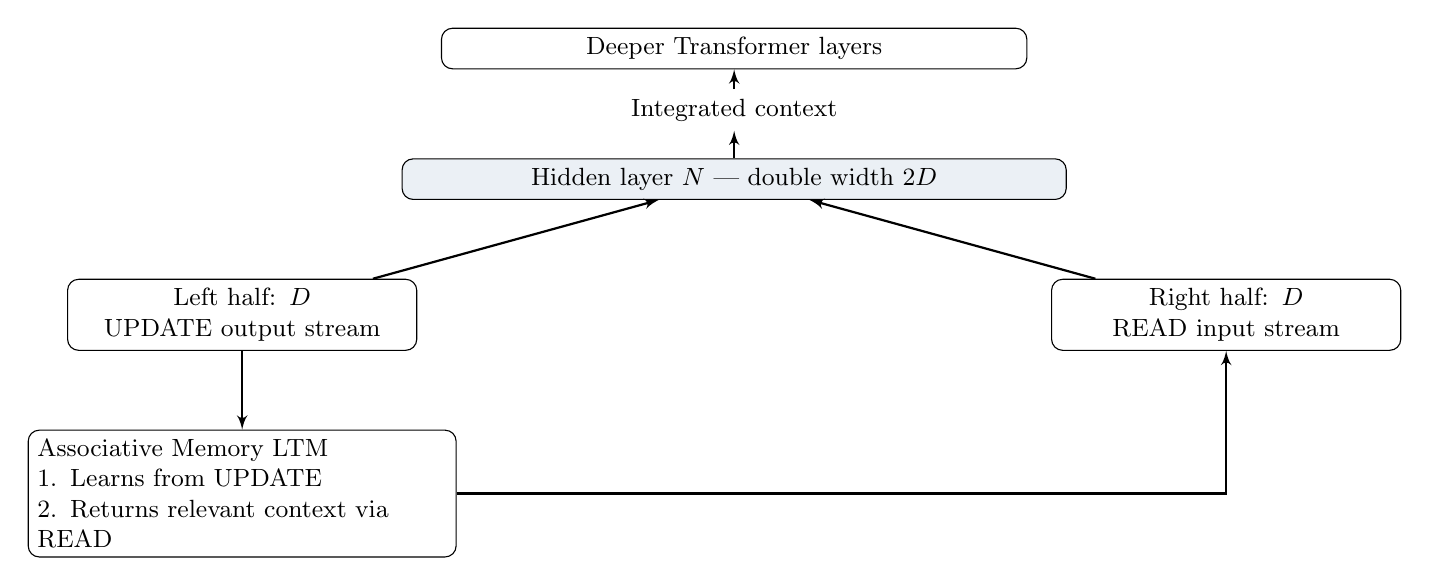
\begin{tikzpicture}[node distance=0.9cm and 1.0cm,>=latex',every node/.style={font=\small}]
\node[draw,rounded corners,align=center,text width=7.2cm](deep){Deeper Transformer layers};
\node[below=0.25cm of deep](ctx){Integrated context};
\node[draw,rounded corners,below=0.35cm of ctx,align=center,text width=8.2cm,fill=secondarycolor](layer){Hidden layer $N$ --- double width $2D$};
\node[draw,rounded corners,below left=1.0cm and -0.2cm of layer,align=center,text width=4.2cm](upd){Left half: $D$\\UPDATE output stream};
\node[draw,rounded corners,below right=1.0cm and -0.2cm of layer,align=center,text width=4.2cm](read){Right half: $D$\\READ input stream};
\node[draw,rounded corners,below=1.0cm of upd,align=left,text width=5.2cm](ltm2){Associative Memory LTM\\1. Learns from UPDATE\\2. Returns relevant context via READ};
\draw[->,thick](layer)--(ctx); \draw[->,thick](ctx)--(deep); \draw[->,thick](upd)--(ltm2);
\draw[->,thick](ltm2.east)-|(read.south); \draw[->,thick](upd)--(layer); \draw[->,thick](read)--(layer);
\end{tikzpicture}
\caption{Double-width layer as a neural UPDATE/READ bus.}
\end{figure}

\subsubsection*{Architectural Advantages of the Scheme}
\begin{enumerate}
\item \textbf{Closed-Loop Perception--Action:}
\begin{itemize}
\item the left half expresses the Transformer's current internal state or intent (UPDATE), transmitting it to LTM in the internal language;
\item the right half receives the memory response (READ), containing associated patterns from LTM-1 and LTM-2;
\item deeper Transformer layers combine both representations $[\mathrm{UPDATE}\parallel\mathrm{READ}]$, integrating memory into reasoning and answer generation.
\end{itemize}
\item \textbf{No decoding delay:} memory does not need to convert the retrieved structure back into text. LTM accepts an UPDATE vector and returns the corresponding vector or mixture of vectors through READ. The Transformer receives the response in its native form.
\item \textbf{Synchronous interaction:} because UPDATE and READ share the same internal interface, memory acts not as an external database but as an extension of latent working space (Latent Coprocessor).
\end{enumerate}

\subsubsection*{Key Challenges and Bottlenecks}
\paragraph{2. Channel Balancing (Attention Masking / Gating).}
\textbf{Problem:} during early LTM training, the READ channel may return noise. If deep Transformer layers fully consume this channel, memory noise can disrupt the base model's linguistic coherence.

\textbf{Solution:} introduce a gating mechanism between channels:
\begin{equation}
\mathrm{Layer}_{out}=W_1\cdot\mathrm{UPDATE}+\sigma\!\left(W_g\cdot[\mathrm{UPDATE},\mathrm{READ}]\right)\odot\left(W_2\cdot\mathrm{READ}\right).
\end{equation}
The gate $\sigma$ learns how strongly the deeper layers should trust READ depending on context.

\paragraph{3. Gradient Stability during Offline Learning.}
If LTM learns autonomously during a Sleep phase and restructures LTM-1/LTM-2, the distribution of signals entering READ changes. To keep deep Transformer layers from depending on uncontrolled distribution drift, READ should pass through LayerNorm with a fixed distribution.

\subsubsection*{Summary of Model Evolution}
\begin{enumerate}
\item The LLM / Transformer acts as a universal cognitive processor.
\item Double-width layer $N$ acts as a neural bus: the right half receives context from past episodes and the left half transmits the current state.
\item In offline Sleep, LTM-2 is compressed, unimportant details are removed, or entire episodes are forgotten, preventing uncontrolled growth and forming abstractions.
\end{enumerate}

\subsubsection*{Dialogue Session Lifecycle}
The first external request tells memory that a dialogue must begin. The next request activates the existing dialogue and, within it, forms a message for the Transformer. When a new request reaches the target Transformer layer, it generates an update that changes the dialogue context for subsequent requests and records the new state in memory.

\begin{figure}[H]
\centering
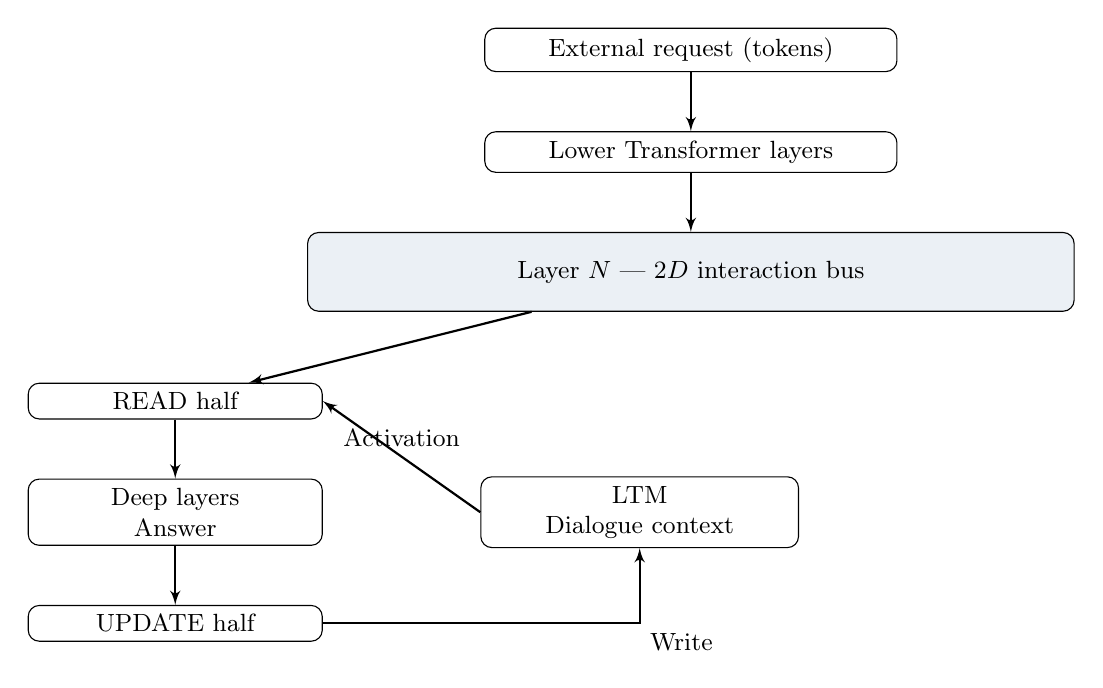
\begin{tikzpicture}[node distance=0.75cm and 1.0cm,>=latex',every node/.style={font=\small}]
\node[draw,rounded corners,align=center,text width=5.0cm](req){External request (tokens)};
\node[draw,rounded corners,below=of req,align=center,text width=5.0cm](low){Lower Transformer layers};
\node[draw,rounded corners,below=of low,align=center,text width=9.5cm,minimum height=1.0cm,fill=secondarycolor](bus){Layer $N$ --- $2D$ interaction bus};
\node[draw,rounded corners,below left=0.9cm and -0.2cm of bus,align=center,text width=3.5cm](read2){READ half};
\node[draw,rounded corners,below=of read2,align=center,text width=3.5cm](deep2){Deep layers\\Answer};
\node[draw,rounded corners,below=of deep2,align=center,text width=3.5cm](upd2){UPDATE half};
\node[draw,rounded corners,right=2.0cm of deep2,align=center,text width=3.8cm](ctx2){LTM\\Dialogue context};
\draw[->,thick](req)--(low); \draw[->,thick](low)--(bus); \draw[->,thick](bus)--(read2);
\draw[->,thick](read2)--(deep2); \draw[->,thick](deep2)--(upd2);
\draw[->,thick](upd2.east)-|node[below right]{Write}(ctx2.south); \draw[->,thick](ctx2.west)--node[above]{Activation}(read2.east);
\end{tikzpicture}
\caption{Stepwise READ/UPDATE cycle within an active dialogue.}
\end{figure}

\paragraph{Step 1: Initialization (first external request).}
\begin{enumerate}
\item \textbf{Input:} an external request enters the system.
\item \textbf{Start signal:} the lower Transformer layers reach layer $N$; UPDATE generates a ``Start dialogue'' trigger vector.
\item \textbf{Associative-memory response:} LTM recognizes the trigger, creates a new session node/context in LTM-2, and initializes READ.
\item \textbf{Result:} a pointer to the new dialogue is created and memory is ready to accumulate the episode.
\end{enumerate}

\paragraph{Step 2: Active Phase (each subsequent request).}
\textbf{1. Reading existing context (READ Phase):}
\begin{itemize}
\item a new user request enters the Transformer;
\item on reaching layer $N$, the system takes the current dialogue-graph state from LTM-2 and feeds its latent representation into READ;
\item deeper Transformer layers receive a memory vector compressing previous facts, roles, and dialogue context;
\item the Transformer generates a response to the user.
\end{itemize}
\textbf{2. Writing and updating context (UPDATE Phase):}
\begin{itemize}
\item UPDATE sends LTM the revised internal state: what happened, which LTM-1 concepts were involved, and the new causal step;
\item LTM consumes UPDATE and extends the current dialogue graph in LTM-2, linking the new step to previous ones.
\end{itemize}

\paragraph{Step 3: Consolidation (session end / transition to Sleep).}
When the dialogue stops, the accumulated LTM-2 session graph is marked as a Completed Logical Episode. During Sleep the episode graph is consolidated: association weights in LTM-1 are updated, while the LTM-2 dialogue graph is generalized and compressed into long-term experience.

\subsubsection*{Architectural Consequences}
\begin{enumerate}
\item \textbf{The Transformer context window becomes practically ``infinite'':} the Transformer need not retain the entire previous text in the standard Attention window; it receives a compressed state of the current dialogue from LTM via READ.
\item \textbf{Memory as a State Machine:} LTM is not static storage but a dynamic neural state environment. Every UPDATE moves the dialogue graph from $\mathrm{State}_t$ to $\mathrm{State}_{t+1}$.
\item \textbf{Dialogue locality in LTM-2:} each active dialogue forms a temporary branch or subgraph in LTM-2 connected to base LTM-1 elements.
\end{enumerate}

\paragraph{Start-Signal Clarification.}
The start signal is the arrival of a signal at the Transformer's input layer. A new dialogue that has not yet received any update generates no read. This sets a strict initialization boundary condition: if the dialogue is empty, the system has nothing on which to perform associative search in LTM.

\subsection*{Two-Stage Cold-Start Protocol}
To avoid using a dialogue context that has not yet been formed, interaction starts in two stages:
\begin{itemize}
\item \textbf{Turn $T_1$ --- initialization.} The hidden state of the first message initializes and anchors D-Context. Feedback injection is disabled: $\Delta h_{T_1}=\mathbf 0$.
\item \textbf{Turn $T_2+$ --- active interaction.} Beginning with the second message, associative memory uses accumulated D-Context to retrieve relevant information; returned state $\Delta h_{T_n}$ is reintegrated into the Transformer Residual Stream.
\end{itemize}

\subsection*{End-to-End Reintegration}
After the state is modified at $l_{\text{target}}^{\text{out}}$, subsequent Transformer layers operate normally. Over a small number of additional layers introduced together with the doubling of $l_{\text{target}}$, information returned by memory should smoothly merge into the common stream and participate in all subsequent computations up to output-logit formation:
\begin{equation}
h_t^{(l)}=h_t^{(l-1)}+\operatorname{SelfAttention}^{(l)}\!\left(\operatorname{LN}(h_t^{(l-1)})\right)+\operatorname{MLP}^{(l)}\!\left(\operatorname{LN}(h_t^{(l-1)})\right),
\end{equation}
\begin{equation}
P(y_t\mid y_{<t})=\operatorname{Softmax}\!\left(W_{\text{head}}\operatorname{LN}(h_t^{(L)})\right).
\end{equation}

\section{Automatic Layer Selection (Layer Entropy Profiling)}
Hidden states $h_t^{(l)}\in\mathbb{R}^d$ change their functional nature radically with network depth $l\in[1,L]$. Early layers are saturated with surface syntactic noise, while the deepest layers exhibit representation degeneration before tokenizer projection.

To avoid heuristic layer selection, a \textbf{Layer Entropy Profiler} is used:
\begin{figure}[H]
\centering
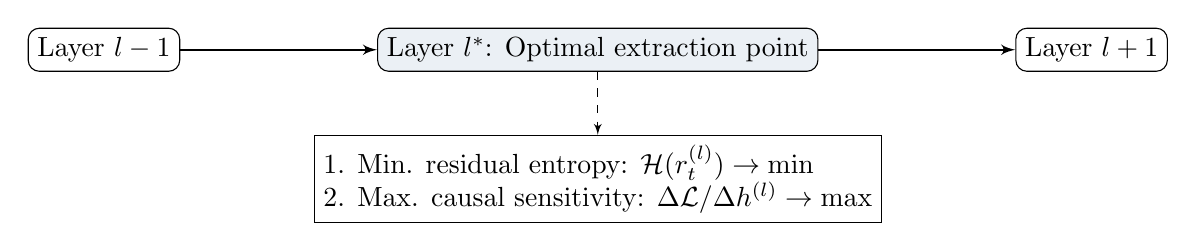
\begin{tikzpicture}[node distance=2.5cm,auto,>=latex']
\node[draw,rectangle,rounded corners](l1){Layer $l-1$};
\node[draw,rectangle,rounded corners,fill=secondarycolor,right=of l1](l){Layer $l^*$: Optimal extraction point};
\node[draw,rectangle,rounded corners,right=of l](l2){Layer $l+1$};
\draw[->,thick](l1)--(l); \draw[->,thick](l)--(l2);
\node[draw,rectangle,fill=white,below=0.8cm of l,align=left](info){1. Min. residual entropy: $\mathcal{H}(r_t^{(l)})\to\min$\\2. Max. causal sensitivity: $\Delta\mathcal L/\Delta h^{(l)}\to\max$};
\draw[->,dashed](l)--(info);
\end{tikzpicture}
\end{figure}

\subsection*{Mathematical Criterion}
The optimal layer index $l^*$ is defined as the global minimum of the differential entropy of residual-vector distributions subject to exceeding the task's causal-sensitivity threshold:
\begin{equation}
l^*=\arg\min_{l\in[1,L]}\mathcal H\!\left(h^{(l)}-\mathbf P_{\mathcal B}h^{(l)}\right)\quad\text{subject to}\quad
\mathbb E\!\left[\left\|\frac{\partial\mathcal L_{\text{task}}}{\partial h^{(l)}}\right\|\right]>\tau_{\text{causal}}.
\end{equation}
where $\mathcal H(\cdot)$ is differential entropy and $\mathbf P_{\mathcal B}$ is the projection operator onto the current basis.

\clearpage
\phantomsection
\addcontentsline{toc}{section}{One Possible Implementation of the Above}
\begin{center}
{\Huge\bfseries One Possible Implementation of the Above\par}
\end{center}
\vspace{0.8cm}

At the beginning of this document, we promised to \textbf{show how the system's associative memory can learn this language and use it}.

Everything below is one possible way of doing so. This section contains a great deal of mathematics and no new conceptual ideas; it can therefore be skipped without compromising the general understanding of the concept.

Most of the work described below is performed offline and requires only administrative access to an already trained Transformer model that will subsequently be used in the Cognitive system. The existing Transformer is used to generate the required statistics from datasets that will then be processed by the algorithms described below. For example, books passed through the Transformer can be grouped by genre and author, paintings by artist, and landscape photographs by landscape type, and so on.

The resulting large body of structured data will be used by the algorithms described below to determine the semantics of the internal language.

\footnotesize
\section{Stage I: Extracting the Asemantic Physical Basis $\mathcal{B}$}
At the first stage, the system is isolated from notions of semantics and meaning. The statistical geometry of activation distributions is analyzed across a set of heterogeneous text domains $g\in G$.

\begin{center}
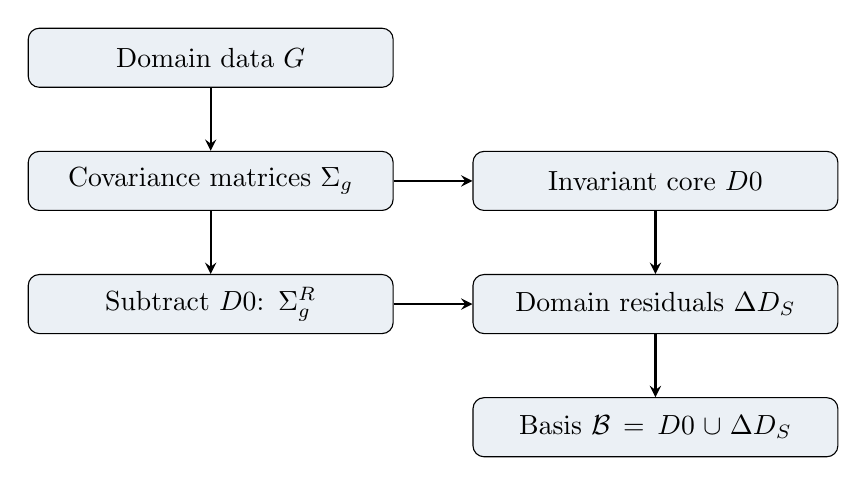
\begin{tikzpicture}[node distance=0.8cm and 1.0cm,box/.style={draw,rounded corners,align=center,minimum height=0.75cm,text width=4.4cm,fill=secondarycolor},arr/.style={->,>=stealth,thick}]
\node[box](domains){Domain data $G$}; \node[box,below=of domains](cov){Covariance matrices $\Sigma_g$};
\node[box,right=of cov](core){Invariant core $D0$}; \node[box,below=of cov](res){Subtract $D0$: $\Sigma_g^R$};
\node[box,right=of res](delta){Domain residuals $\Delta D_S$}; \node[box,below=of delta](basis){Basis $\mathcal B=D0\cup\Delta D_S$};
\draw[arr](domains)--(cov); \draw[arr](cov)--(core); \draw[arr](cov)--(res); \draw[arr](core)--(delta); \draw[arr](res)--(delta); \draw[arr](delta)--(basis);
\end{tikzpicture}
\end{center}

\subsection*{Computation Algorithm}
\begin{enumerate}
\item \textbf{Activation covariance collection:} at tap layer $l^*$, a covariance matrix is collected for each domain:
\begin{equation}\Sigma_g=\frac1{N_g}\sum_{t=1}^{N_g}(h_t^g-\bar h^g)(h_t^g-\bar h^g)^T\in\mathbb R^{d\times d}.\end{equation}
\item \textbf{Central syntax invariant extraction ($D0$):} form $\Sigma_{\text{mean}}=\frac1{|G|}\sum_{g=1}^{|G|}\Sigma_g$. Spectral decomposition (SVD) extracts the first $k_0$ principal vectors, defining the orthonormal core $D0$.
\item \textbf{Specialized dictionary extraction ($\Delta D_S$):} for each domain, compute a residual covariance matrix with the influence of $D0$ completely removed by orthogonal projection:
\begin{equation}\Sigma_g^R=(I-P_{D0})\Sigma_g(I-P_{D0})^T,\qquad \text{where }P_{D0}=D0\,D0^T.\end{equation}
The top-$k_s$ vectors are selected from the SVD $\Sigma_g^R=U_g\Lambda_gU_g^T$.
\item \textbf{Frozen basis formation:}
\begin{equation}\mathcal B=D0\cup\left(\bigcup_{g\in G}\Delta D_{S,g}\right)=\{d_1,d_2,\dots,d_M\}\subset\mathbb R^d.\end{equation}
All vectors are normalized, $\|d_k\|_2=1$. This basis is fixed as the universal coordinate grid.
\end{enumerate}

\section{Stage II: Causal-Interventional Verification (Causal Patching)}
Each basis vector $d_k\in\mathcal B$ is tested for functional efficacy by two opposite mathematical interventions in the neural network.
\begin{center}
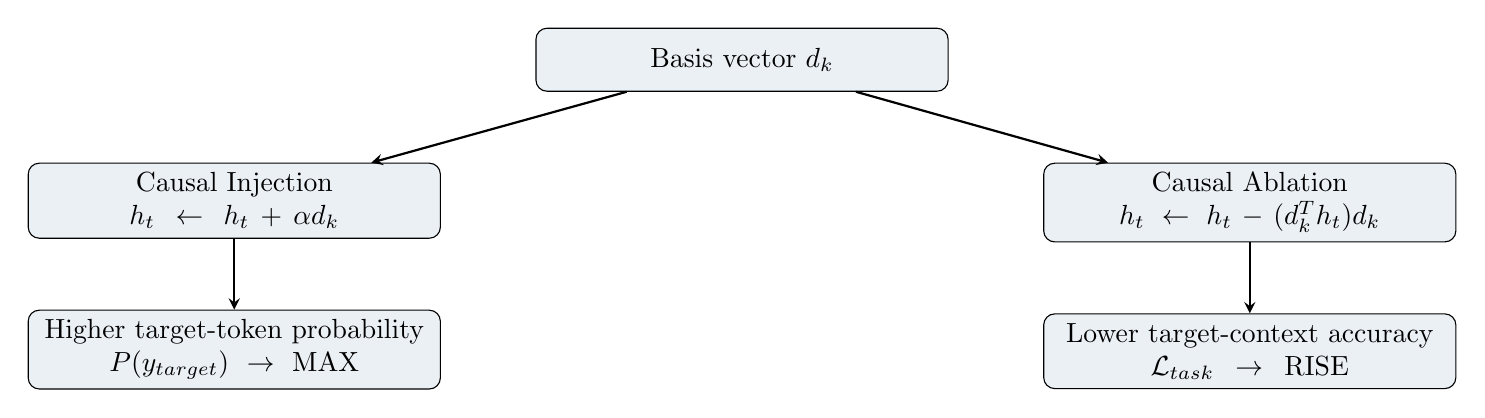
\begin{tikzpicture}[node distance=0.9cm and 1.2cm,box/.style={draw,rounded corners,align=center,minimum height=0.8cm,text width=5.0cm,fill=secondarycolor},arr/.style={->,>=stealth,thick}]
\node[box](v){Basis vector $d_k$}; \node[box,below left=of v](inj){Causal Injection\\$h_t\leftarrow h_t+\alpha d_k$};
\node[box,below right=of v](abl){Causal Ablation\\$h_t\leftarrow h_t-(d_k^Th_t)d_k$};
\node[box,below=of inj](inc){Higher target-token probability\\$P(y_{target})\rightarrow\mathrm{MAX}$};
\node[box,below=of abl](dec){Lower target-context accuracy\\$\mathcal L_{task}\rightarrow\mathrm{RISE}$};
\draw[arr](v)--(inj); \draw[arr](v)--(abl); \draw[arr](inj)--(inc); \draw[arr](abl)--(dec);
\end{tikzpicture}
\end{center}
\begin{enumerate}
\item \textbf{Causal Injection:} in a neutral context at $l^*$, inject $h_t\leftarrow h_t+\alpha d_k$. The vector is considered causally active if the output-layer $W_{\text{unembed}}$ logit shift produces a statistically significant probability increase for a specific token group.
\item \textbf{Causal Ablation:} in a context where the vector is naturally active, null it via $h_t\leftarrow h_t-(d_k^Th_t)d_k$. Retain it only if subtraction causally changes model behavior, $\Delta\mathcal L_{\text{task}}>\tau$.
\end{enumerate}

\section{Stage III: Task Reduction and Construction of Semantic Graph $G_T$}
For a downstream task $T$, the model produces an activation sequence $H_T=\{h_1,h_2,\dots,h_N\}\subset\mathbb R^d$. Each vector is decomposed over the frozen basis, $h_t=\sum_{k=1}^M c_{t,k}d_k+r_t$, where $c_{t,k}=h_t^Td_k$.

\subsection*{A. Semantic Filtering (Pruning)}
The universal dictionary is compressed into the task-specific functional semantic dictionary $\mathcal V_T\subset\mathcal B$:
\begin{equation}\mathcal V_T=\left\{d_k\in\mathcal B\;\middle|\;\frac1N\sum_{t=1}^N|h_t^Td_k|>\tau_E\;\land\;\Delta\mathcal L_T(d_k)>\tau_L\right\}.\end{equation}
Vectors with low projection energy and zero causal influence are discarded.

\subsection*{B. Semantic Edge Induction}
To turn $\mathcal V_T$ into a \textbf{Directed Semantic Graph $G_T=(\mathcal V_T,E_T,W)$}, two kinds of relationships are computed between nodes $d_i$ and $d_j$:
\begin{enumerate}
\item \textbf{Synchronic Co-activation:}
\begin{equation}W_{ij}^{\text{co}}=\frac{\sum_{t=1}^N(c_{t,i}-\bar c_i)(c_{t,j}-\bar c_j)}{\sqrt{\sum_t(c_{t,i}-\bar c_i)^2\sum_t(c_{t,j}-\bar c_j)^2}}.\end{equation}
\item \textbf{Diachronic Causal Flow ($t\rightarrow t+1$):}
\begin{equation}W_{i\to j}^{\text{causal}}=\frac1{N-1}\sum_{t=1}^{N-1}c_{t,i}c_{t+1,j}.\end{equation}
\end{enumerate}
The final directed edge weight is $W_{ij}=\alpha W_{ij}^{\text{co}}+\beta W_{i\to j}^{\text{causal}}$.

\section{Automatic Node Annotation (NodeAnnotator)}
Abstract vectors are converted into a human-readable knowledge map by a three-stage annotation module:
\begin{center}
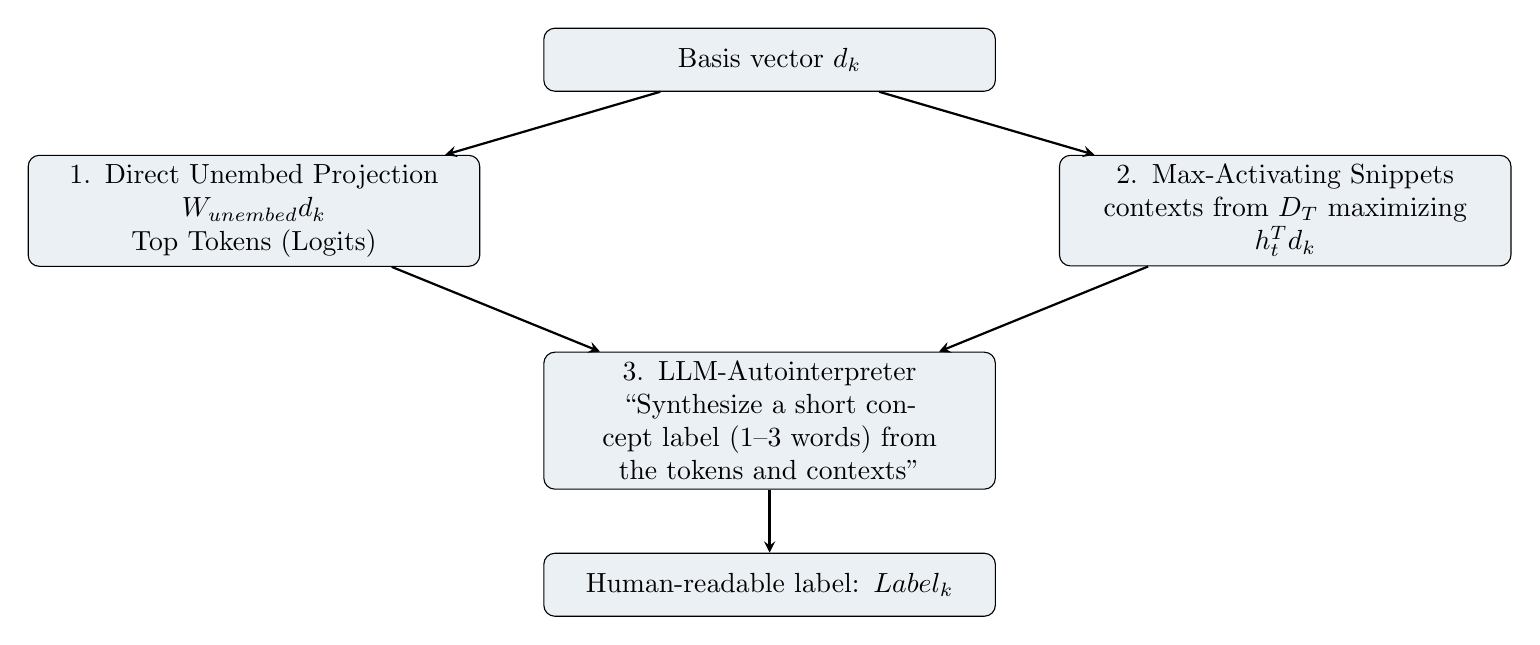
\begin{tikzpicture}[node distance=0.8cm and 0.8cm,box/.style={draw,rounded corners,align=center,minimum height=0.8cm,text width=5.5cm,fill=secondarycolor},arr/.style={->,>=stealth,thick}]
\node[box](v){Basis vector $d_k$}; \node[box,below left=of v](u){1. Direct Unembed Projection\\$W_{unembed}d_k$\\Top Tokens (Logits)};
\node[box,below right=of v](s){2. Max-Activating Snippets\\contexts from $D_T$ maximizing\\$h_t^Td_k$};
\node[box,below=1.1cm of v,yshift=-2.2cm](llm){3. LLM-Autointerpreter\\``Synthesize a short concept label (1--3 words) from the tokens and contexts''};
\node[box,below=of llm](lab){Human-readable label: $Label_k$};
\draw[arr](v)--(u); \draw[arr](v)--(s); \draw[arr](u)--(llm); \draw[arr](s)--(llm); \draw[arr](llm)--(lab);
\end{tikzpicture}
\end{center}
\begin{enumerate}
\item \textbf{Direct Unembedding Projection:} top vocabulary tokens are obtained through $z_k=W_{\text{unembed}}d_k$.
\item \textbf{Max-Activating Dataset Snippets:} select training contexts producing the maximum projection amplitude $c_{t,k}$.
\item \textbf{LLM-Autointerpreter:} a lightweight interpreter generates strict JSON with a human-readable label (e.g. \texttt{Label: "Integral convergence condition"}).
\end{enumerate}

\section{Stage IV: Dynamic Memory Expansion under World Change (OOD Induction)}
When fundamentally new real-world phenomena appear (Concept Drift), hidden states $h_t$ can no longer be decomposed losslessly over the frozen basis $\mathcal B$.

\subsection*{1. Out-Of-Distribution (OOD) Detection}
Monitor the critical residual-energy level:
\begin{equation}r_t=h_t-\sum_{k=1}^M(h_t^Td_k)d_k\quad\Longrightarrow\quad\text{OOD criterion: }\frac{\|r_t\|_2^2}{\|h_t\|_2^2}>\tau_{\text{OOD}}.\end{equation}
Persistent residuals are placed in a ring buffer $R\in\mathbb R^{P\times d}$.
\begin{center}
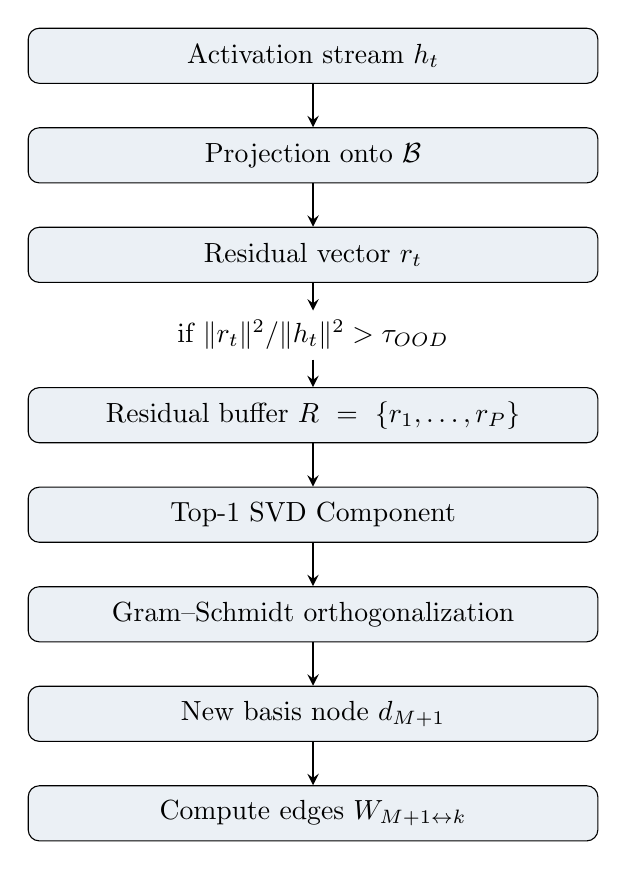
\begin{tikzpicture}[node distance=0.55cm,box/.style={draw,rounded corners,align=center,minimum height=0.7cm,text width=7.0cm,fill=secondarycolor},arr/.style={->,>=stealth,thick}]
\node[box](h){Activation stream $h_t$}; \node[box,below=of h](p){Projection onto $\mathcal B$}; \node[box,below=of p](r){Residual vector $r_t$};
\node[align=center,below=0.35cm of r](q){if $\|r_t\|^2/\|h_t\|^2>\tau_{OOD}$}; \node[box,below=0.35cm of q](buf){Residual buffer $R=\{r_1,\ldots,r_P\}$};
\node[box,below=of buf](svd){Top-1 SVD Component}; \node[box,below=of svd](gs){Gram--Schmidt orthogonalization};
\node[box,below=of gs](new){New basis node $d_{M+1}$}; \node[box,below=of new](edge){Compute edges $W_{M+1\leftrightarrow k}$};
\draw[arr](h)--(p); \draw[arr](p)--(r); \draw[arr](r)--(q); \draw[arr](q)--(buf); \draw[arr](buf)--(svd); \draw[arr](svd)--(gs); \draw[arr](gs)--(new); \draw[arr](new)--(edge);
\end{tikzpicture}
\end{center}

\subsection*{2. New Item and Relationship Induction Algorithm}
\begin{enumerate}
\item \textbf{Geometry extraction:} from residual buffer $R$, extract $d_{\text{raw}}=\text{Top-1 SVD}(R)$.
\item \textbf{Gram--Schmidt orthogonalization:} subtract projections onto all existing basis vectors:
\begin{equation}d_{\text{orth}}=d_{\text{raw}}-\sum_{k=1}^M(d_{\text{raw}}^Td_k)d_k,\qquad d_{M+1}=\frac{d_{\text{orth}}}{\|d_{\text{orth}}\|_2}.\end{equation}
\item \textbf{Basis expansion:} $\mathcal B_{\text{new}}=\mathcal B\cup\{d_{M+1}\}$.
\item \textbf{Graph $G_T$ edge integration:} \texttt{DynamicEdgeIntegrator} computes synchronic and causal relationships between new node $M+1$ and active graph nodes from buffered contexts.
\end{enumerate}

\section{Software Implementation: \texttt{AssociativeMemoryEngine} Module}
The Python code below demonstrates the complete OOD-detection, item-induction, and dynamic edge-construction pipeline:
\begin{lstlisting}
import torch
import torch.nn as nn
import networkx as nx

class AssociativeMemoryEngine(nn.Module):
    def __init__(self, frozen_basis: torch.Tensor, ood_threshold: float = 0.2,
                 buffer_capacity: int = 100, device: str = "cuda"):
        super().__init__()
        self.device = device
        self.ood_threshold = ood_threshold
        self.capacity = buffer_capacity
        # Normalized asemantic basis B [M, d]
        self.B = nn.Parameter(torch.nn.functional.normalize(frozen_basis, p=2, dim=1).to(device), requires_grad=False)
        self.residual_buffer = []

    @torch.no_grad()
    def process_step(self, h_t: torch.Tensor) -> tuple[torch.Tensor, torch.Tensor]:
        """Accept activation h_t [batch, d]; return C [batch, M] and R_t [batch, d]."""
        C = torch.matmul(h_t, self.B.T)
        h_reconstructed = torch.matmul(C, self.B)
        R_t = h_t - h_reconstructed
        energy_h = torch.norm(h_t, dim=-1) ** 2
        energy_r = torch.norm(R_t, dim=-1) ** 2
        ratio = energy_r / (energy_h + 1e-8)
        ood_mask = ratio > self.ood_threshold
        if torch.any(ood_mask):
            for r_vec in R_t[ood_mask]: self.residual_buffer.append(r_vec.cpu())
        return C, R_t

    @torch.no_grad()
    def try_induction_new_item(self, graph: nx.DiGraph, edge_threshold: float = 0.15) -> tuple[nx.DiGraph, int | None]:
        if len(self.residual_buffer) < self.capacity: return graph, None
        R_mat = torch.stack(self.residual_buffer[:self.capacity]).to(self.device)
        _, _, Vh = torch.linalg.svd(R_mat, full_matrices=False)
        d_raw = Vh[0]
        proj = torch.matmul(self.B, d_raw)
        d_orth = d_raw - torch.matmul(proj, self.B)
        norm_val = torch.norm(d_orth)
        if norm_val < 1e-5:
            self.residual_buffer.clear(); return graph, None
        d_new = (d_orth / norm_val).unsqueeze(0)
        new_node_id = self.B.shape[0]
        self.B = nn.Parameter(torch.cat([self.B.data, d_new], dim=0), requires_grad=False)
        active_nodes = list(graph.nodes())
        graph.add_node(new_node_id, label=f"OOD_Concept_{new_node_id}")
        if active_nodes:
            c_new = torch.matmul(R_mat, d_new.T).squeeze()
            active_basis = self.B[active_nodes]
            C_act = torch.matmul(R_mat, active_basis.T)
            c_new_c = c_new - c_new.mean()
            C_act_c = C_act - C_act.mean(dim=0, keepdim=True)
            cov = torch.matmul(c_new_c.unsqueeze(0), C_act_c).squeeze(0) / (self.capacity - 1)
            std_prod = (c_new.std() + 1e-8) * (C_act.std(dim=0) + 1e-8)
            W_corr = cov / std_prod
            W_np = W_corr.cpu().numpy()
            for i, target_node in enumerate(active_nodes):
                if abs(W_np[i]) > edge_threshold:
                    graph.add_edge(target_node, new_node_id, weight=float(W_np[i]))
                    graph.add_edge(new_node_id, target_node, weight=float(W_np[i]))
        self.residual_buffer.clear()
        return graph, new_node_id
\end{lstlisting}

\subsection*{Integration Example: \texttt{TransformerMemoryPipeline}}
The following simplified module illustrates the complete state-read path, two-stage D-Context startup, and reintegration of latent memory state into subsequent Transformer layers:
\begin{lstlisting}
class TransformerMemoryPipeline(nn.Module):
    def __init__(self, transformer_layers, frozen_basis, extract_idx, inject_idx, device="cuda"):
        super().__init__(); self.layers=transformer_layers; self.extract_idx=extract_idx; self.inject_idx=inject_idx
        self.B=nn.Parameter(torch.nn.functional.normalize(frozen_basis,p=2,dim=1).to(device),requires_grad=False)
        self.turn_counter=0; self.d_context_vector=torch.zeros(frozen_basis.shape[1],device=device)

    def start_new_dialogue(self):
        self.turn_counter=0; self.d_context_vector.zero_()

    def forward(self, hidden_states):
        self.turn_counter += 1; delta_h=None
        for idx, layer in enumerate(self.layers):
            # Input Pole: extract state
            if idx == self.extract_idx:
                h_extract=hidden_states.clone(); coeff=torch.matmul(h_extract,self.B.T); h_proj=torch.matmul(coeff,self.B)
                if self.turn_counter == 1:
                    self.d_context_vector=h_proj.mean(dim=0); delta_h=torch.zeros_like(hidden_states)
                else:
                    self.d_context_vector=0.85*self.d_context_vector+0.15*h_proj.mean(dim=0)
                    delta_h=(h_proj*0.10)+(self.d_context_vector*0.05)
            hidden_states=layer(hidden_states)
            # Output Pole: reintegrate into the Residual Stream
            if idx == self.inject_idx and delta_h is not None: hidden_states=hidden_states+delta_h
        return hidden_states
\end{lstlisting}

The code above illustrates the interface rather than the final retrieval implementation: in the complete architecture, $\Delta h_t$ must be formed by associative memory from the query, D-Context, and active graph $G_T$.

\section{Two-Stage System Architecture}
The architecture separates the construction of a stable physical basis from the task-dependent construction of semantic structure.
\begin{figure}[H]
\centering
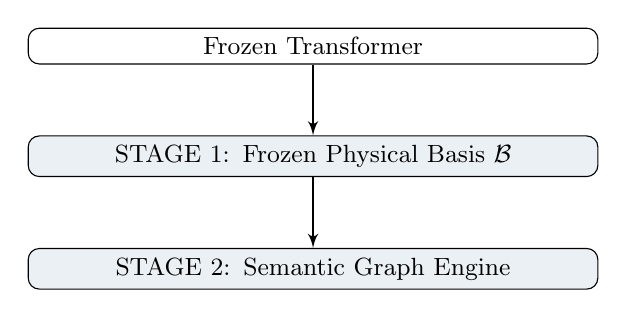
\begin{tikzpicture}[node distance=0.9cm,>=latex',every node/.style={font=\small}]
\node[draw,rounded corners,align=center,text width=7.0cm](tr){Frozen Transformer};
\node[draw,rounded corners,below=of tr,fill=secondarycolor,align=center,text width=7.0cm](stage1){STAGE 1: Frozen Physical Basis $\mathcal B$};
\node[draw,rounded corners,below=of stage1,fill=secondarycolor,align=center,text width=7.0cm](stage2){STAGE 2: Semantic Graph Engine};
\draw[->,thick](tr)--(stage1); \draw[->,thick](stage1)--(stage2);
\end{tikzpicture}
\caption{Two-stage system: a frozen physical basis and a dynamic Semantic Graph Engine.}
\end{figure}

\subsection*{Mathematical Apparatus of Stage 2}
For a task $T$, let the sequence of hidden activations be
\[H_T=\{h_1,h_2,\dots,h_N\}.\]
Each vector is decomposed over the frozen basis $\mathcal B$:
\[h_t=\sum_{k=1}^{M}c_{t,k}d_k+r_t,\qquad c_{t,k}=h_t^Td_k.\]

\subsubsection*{Step A. Semantic Filtering (Pruning \& Sparsification)}
A vector $d_k\in\mathcal B$ is considered an active semantic ``word'' for task $T$ when its projection coefficient is not merely geometrically expressed but informationally relevant to solving the task.
\begin{enumerate}
\item \textbf{Activation Energy:} $E_T(d_k)=\frac1N\sum_{t=1}^N|h_t^Td_k|$.
\item \textbf{Task-Specific Ablation Sensitivity:} subtract direction $d_k$ while solving $T$ and measure the increase in task loss $\Delta\mathcal L_T(d_k)$.
\item \textbf{Masking filter:}
\[\mathcal V_T=\{d_k\in\mathcal B\mid E_T(d_k)>\tau_E\land\Delta\mathcal L_T(d_k)>\tau_L\}.\]
All vectors in $\mathcal B\setminus\mathcal V_T$ are removed from the computation for the specific task $T$.
\end{enumerate}

\subsubsection*{Step B. Semantic Edges Induction}
To convert $\mathcal V_T$ into a semantic graph $G_T=(\mathcal V_T,E,W)$, an adjacency matrix is computed between $d_i$ and $d_j$ using three edge types:
\begin{enumerate}
\item \textbf{Co-activation Edge / Synchronic:}
\[W_{ij}^{co}=\frac{\sum_{t=1}^N(c_{t,i}-\bar c_i)(c_{t,j}-\bar c_j)}{\sqrt{\sum_t(c_{t,i}-\bar c_i)^2\sum_t(c_{t,j}-\bar c_j)^2}}.\]
\item \textbf{Causal Flow Edge / Diachronic:}
\[W_{i\rightarrow j}^{causal}=\frac1{N-\delta}\sum_{t=1}^{N-\delta}c_{t,i}\frac{\partial c_{t+\delta,j}}{\partial c_{t,i}}.\]
\item \textbf{Attention-Mediated Edge:}
\[W_{i\rightarrow j}^{attn}=\sum_{t_1,t_2}A_{t_1,t_2}^{(l)}(h_{t_1}^Td_i)(h_{t_2}^Td_j).\]
\end{enumerate}
The final semantic edge has weight
\[W_{ij}=\alpha W_{ij}^{co}+\beta W_{i\rightarrow j}^{causal}+\gamma W_{i\rightarrow j}^{attn}.\]

\subsection*{Why This Scheme Is More Efficient}
\begin{enumerate}
\item \textbf{Computational economy (Zero Re-Training):} SVD, SAE, or Diffusion Maps need not be repeated for every new task. The geometric physical basis $\mathcal B$ is computed once at Stage I.
\item \textbf{Task-space compression:} instead of analyzing the full $12\,288\times12\,288$ space, a task uses roughly $M_{\text{active}}\approx50\ldots200$ key elements.
\item \textbf{Interpretability and graph coprocessing:} nodes $\mathcal V_T$ represent concepts used by the model and edges represent directed logical transitions.
\item \textbf{Graph Editing:} nodes and edges of $G_T$ can be programmatically suppressed by acting on coefficients $c_{t,k}$, without fine-tuning the general-language basis.
\end{enumerate}

\section{Automatic Annotation of Semantic-Graph Nodes}
Assigning text labels to vectors of the asemantic basis $\mathcal B$ transforms geometric graph $G_T$ into a human-readable knowledge map. An individual $d_k\in\mathcal B$ may correspond not to a single word but to an abstract concept, syntactic role, or complex contextual polysemantic pattern.

\subsection*{Three-Stage Annotation Architecture}
\begin{figure}[H]
\centering
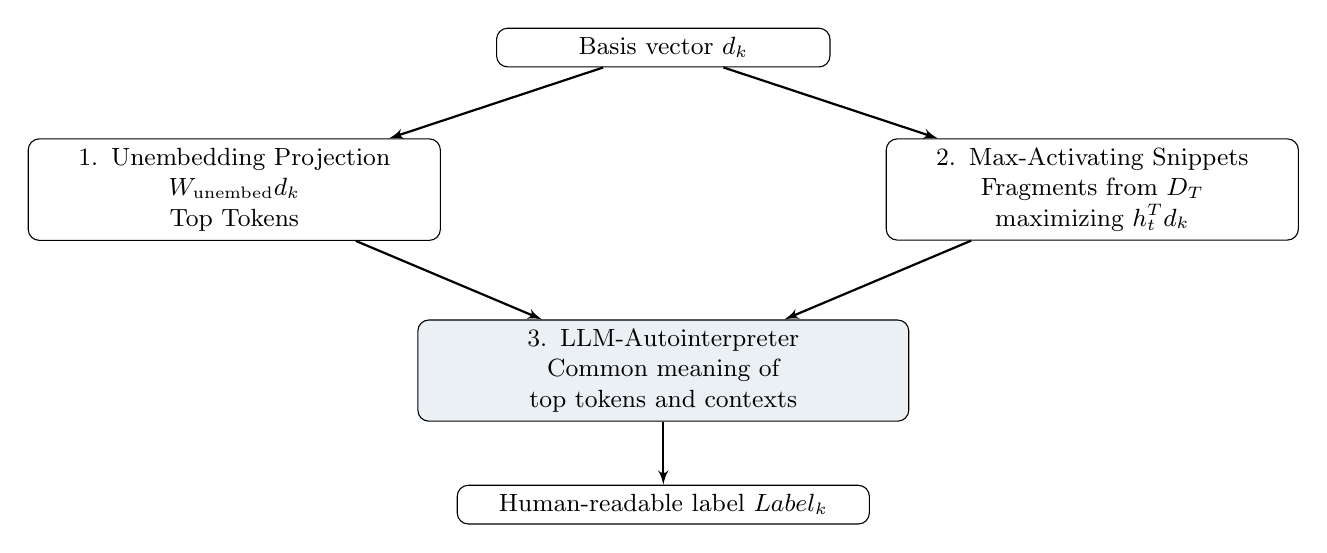
\begin{tikzpicture}[node distance=0.8cm and 1.0cm,>=latex',every node/.style={font=\small}]
\node[draw,rounded corners,align=center,text width=4.0cm](vec){Basis vector $d_k$};
\node[draw,rounded corners,below left=0.9cm and 0.7cm of vec,align=center,text width=5.0cm](unembed){1. Unembedding Projection\\$W_{\text{unembed}}d_k$\\Top Tokens};
\node[draw,rounded corners,below right=0.9cm and 0.7cm of vec,align=center,text width=5.0cm](snip){2. Max-Activating Snippets\\Fragments from $D_T$ maximizing $h_t^Td_k$};
\node[draw,rounded corners,below=1.2cm of vec,yshift=-2.0cm,fill=secondarycolor,align=center,text width=6.0cm](llm){3. LLM-Autointerpreter\\Common meaning of top tokens and contexts};
\node[draw,rounded corners,below=of llm,align=center,text width=5.0cm](label){Human-readable label $Label_k$};
\draw[->,thick](vec)--(unembed); \draw[->,thick](vec)--(snip); \draw[->,thick](unembed)--(llm); \draw[->,thick](snip)--(llm); \draw[->,thick](llm)--(label);
\end{tikzpicture}
\caption{Three-stage automatic annotation of semantic-graph nodes.}
\end{figure}

\subsection*{Detailed Stages}
\paragraph{Stage 1. Projection onto the Vocabulary Unembedding Matrix.}
Project $d_k$ onto $W_{\text{unembed}}\in\mathbb R^{|V|\times d}$:
\[z_k=W_{\text{unembed}}d_k\in\mathbb R^{|V|}.\]
Select Top-$K$ tokens with the largest logits $z_k$, yielding tokens, suffixes, or subwords directly activated by the vector at model output.

\paragraph{Stage 2. Max-Activating Dataset Snippets.}
Run corpus $D_T$ through the model and retain Top-$N$ text fragments maximizing $h_t^Td_k$. The context window around each position reveals abstractions that may not correspond to a single vocabulary token.

\paragraph{Stage 3. LLM-Autointerpretation.}
A compact annotation model receives top tokens and several maximally activating contexts and returns a structured label:
\begin{itemize}
\item \texttt{label}: short concept name;
\item \texttt{category}: ``Concept'', ``Syntax'', ``Style'', or ``Operator'';
\item \texttt{confidence}: confidence estimate.
\end{itemize}

\subsection*{Visual Result of Annotated Graph $G_T$}
After the pipeline, the anonymous vector graph becomes readable:
\begin{itemize}
\item Node \#412 $\rightarrow$ ``Integral computation'' (top tokens: $\int$, integral, dx);
\item Node \#891 $\rightarrow$ ``Convergence condition'' (top tokens: limit, bounded, converges);
\item Edge \#412 $\rightarrow$ \#891 with weight 0.84 means that when the model addresses integrals it causally activates convergence checking.
\end{itemize}
Annotation is performed on demand only for the $M_{\text{active}}$ nodes surviving task-$T$ filtering, reducing LLM-interpreter calls from tens of thousands of basis elements to a few dozen active $G_T$ nodes.

\section{OOD Detection and Dynamic Dictionary Expansion}
New real-world phenomena, terminology, or physical laws (Out-Of-Distribution / Concept Drift) can make the current activation state $h_t\in\mathbb R^d$ impossible to represent losslessly over frozen basis $\mathcal B$. A new object manifests as increased residual $r_t$.

\subsection*{Detection Phase}
\[h_t=\sum_{k=1}^Mc_{t,k}d_k+r_t,\qquad c_{t,k}=h_t^Td_k,\]
\[r_t=h_t-\sum_{k=1}^M(h_t^Td_k)d_k.\]
New-Item detection criteria:
\begin{enumerate}
\item \textbf{High Residual Energy:} $\frac{\|r_t\|_2^2}{\|h_t\|_2^2}>\tau_{\text{OOD}}$, with $\tau_{\text{OOD}}\approx0.15\ldots0.25$.
\item \textbf{Persistent Residual Cluster:} a single outlier is treated as noise. Systematic residual accumulation into a dense cluster in $\mathbb R^d$ indicates a new semantic concept.
\end{enumerate}

\subsection*{Ingestion Phase}
When a stable cluster $R=\{r_1,r_2,\dots,r_P\}$ is detected, Online Incremental Induction begins.
\begin{figure}[H]
\centering
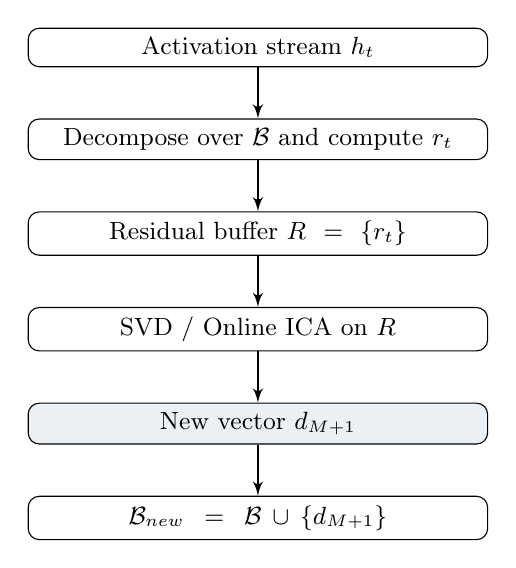
\begin{tikzpicture}[node distance=0.65cm,>=latex',every node/.style={font=\small}]
\node[draw,rounded corners,align=center,text width=5.6cm](act){Activation stream $h_t$};
\node[draw,rounded corners,below=of act,align=center,text width=5.6cm](proj){Decompose over $\mathcal B$ and compute $r_t$};
\node[draw,rounded corners,below=of proj,align=center,text width=5.6cm](buf){Residual buffer $R=\{r_t\}$};
\node[draw,rounded corners,below=of buf,align=center,text width=5.6cm](svd){SVD / Online ICA on $R$};
\node[draw,rounded corners,below=of svd,fill=secondarycolor,align=center,text width=5.6cm](new){New vector $d_{M+1}$};
\node[draw,rounded corners,below=of new,align=center,text width=5.6cm](base){$\mathcal B_{new}=\mathcal B\cup\{d_{M+1}\}$};
\draw[->,thick](act)--(proj); \draw[->,thick](proj)--(buf); \draw[->,thick](buf)--(svd); \draw[->,thick](svd)--(new); \draw[->,thick](new)--(base);
\end{tikzpicture}
\caption{Online induction of a new dictionary element from persistent residuals.}
\end{figure}

\paragraph{Step A. Residual Buffer.} All $r_t$ exceeding $\tau_{\text{OOD}}$ are placed in a ring buffer $R\in\mathbb R^{P\times d}$.

\paragraph{Step B. Extract the New-Concept Direction.} After accumulating $P$ vectors (e.g. $P=100\ldots500$), use $d_{\text{new}}=\operatorname{Top\mbox{-}1\,SVD}(R)$ or the normalized mean of stable residuals.

\paragraph{Step C. Gram--Schmidt Orthogonalization.}
\[d_{\text{new}}^{orth}=d_{\text{new}}-\sum_{k=1}^M(d_{\text{new}}^Td_k)d_k,\qquad d_{M+1}=\frac{d_{\text{new}}^{orth}}{\|d_{\text{new}}^{orth}\|}.\]

\paragraph{Step D. Integration.}
\begin{enumerate}
\item add $d_{M+1}$ to $\mathcal B$: $\mathcal B_{updated}=\mathcal B\cup\{d_{M+1}\}$;
\item NodeAnnotator generates a label from contexts that produced $r_t$;
\item create node $M+1$ in $G_T$ and induce its semantic edges.
\end{enumerate}

\subsection*{Architectural Advantages}
\begin{enumerate}
\item \textbf{Continual Zero-Forgetting Learning:} new data do not retrain the Transformer or alter existing $d_1,\dots,d_M$; a new orthogonal direction $d_{M+1}$ is added.
\item \textbf{Noise vs. new-concept separation:} random fluctuations cancel in the buffer SVD while persistent geometric shifts survive.
\item \textbf{Knowledge-evolution audit:} every new item may receive an induction timestamp, allowing the system's world model to be tracked over time.
\end{enumerate}

\section{Integrating a New Item into the Semantic Graph}
A new vector $d_{M+1}$ in basis $\mathcal B$ is only the physical registration of a novel phenomenon. To make it a full element of model reasoning, semantic edges must be integrated into current graph $G_T$.

\subsection*{Dynamic Edge Induction \& Integration Architecture}
\begin{figure}[H]
\centering
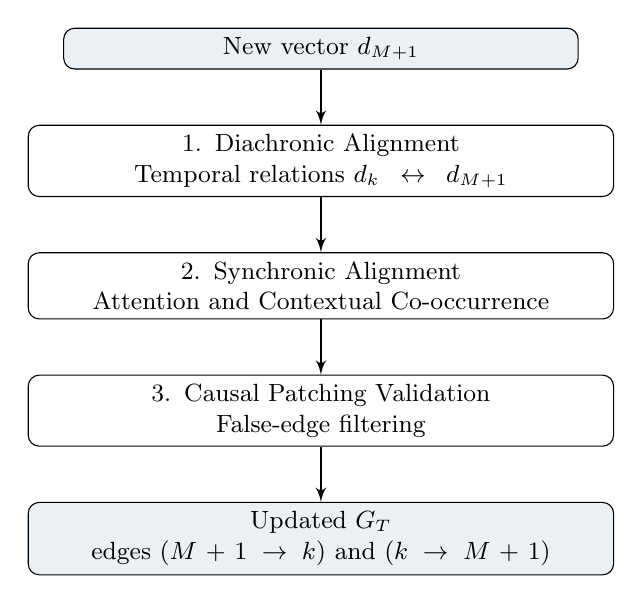
\begin{tikzpicture}[node distance=0.7cm,>=latex',every node/.style={font=\small}]
\node[draw,rounded corners,fill=secondarycolor,align=center,text width=6.3cm](new){New vector $d_{M+1}$};
\node[draw,rounded corners,below=of new,align=center,text width=7.2cm](dia){1. Diachronic Alignment\\Temporal relations $d_k\leftrightarrow d_{M+1}$};
\node[draw,rounded corners,below=of dia,align=center,text width=7.2cm](sync){2. Synchronic Alignment\\Attention and Contextual Co-occurrence};
\node[draw,rounded corners,below=of sync,align=center,text width=7.2cm](patch){3. Causal Patching Validation\\False-edge filtering};
\node[draw,rounded corners,below=of patch,fill=secondarycolor,align=center,text width=7.2cm](graph){Updated $G_T$\\edges $(M+1\rightarrow k)$ and $(k\rightarrow M+1)$};
\draw[->,thick](new)--(dia); \draw[->,thick](dia)--(sync); \draw[->,thick](sync)--(patch); \draw[->,thick](patch)--(graph);
\end{tikzpicture}
\caption{Integration of a new Item into the dynamic semantic graph.}
\end{figure}

\subsection*{Computing Semantic Relationships for $d_{M+1}$}
After forming a new vector from residual buffer $R=\{r_1,r_2,\dots,r_P\}$, retain activation sequences in which the concept appeared. To connect node $M+1$ to each existing active node $k\in G_T$, compute:

\paragraph{1. Forward/Backward Diachronic Flow.}
Incoming edge:
\[W_{k\rightarrow M+1}^{causal}=\frac1{P-1}\sum_{t=1}^{P-1}(h_t^Td_k)(h_{t+1}^Td_{M+1}).\]
Outgoing edge:
\[W_{M+1\rightarrow k}^{causal}=\frac1{P-1}\sum_{t=1}^{P-1}(h_t^Td_{M+1})(h_{t+1}^Td_k).\]

\paragraph{2. Synchronic Context Coupling.}
\[W_{M+1,k}^{co}=\frac{\operatorname{Cov}(h_t^Td_{M+1},h_t^Td_k)}{\sigma(d_{M+1})\sigma(d_k)}.\]

\paragraph{3. Causal Patching for False-Edge Filtering.}
For the highest-weight candidate edges, perform a causal test:
\begin{enumerate}
\item in a context where $d_k$ activates, artificially ablate it;
\item if activation of $d_{M+1}$ on the next step falls by $\Delta>\tau_{\text{causal}}$, accept edge $e(k\rightarrow M+1)$ as causally valid.
\end{enumerate}

\subsection*{Complete Lifecycle Example for a New Item}
If a new vulnerability such as ``DeepSeek-R1 Prompt Injection'' appears in the external world, its lifecycle is:
\begin{enumerate}
\item \textbf{Detection:} $\mathcal B$ cannot fully represent the specific context, so residual $r_t$ grows.
\item \textbf{Induction:} residuals accumulate and SVD extracts orthogonal vector $d_{M+1}$.
\item \textbf{Annotation:} NodeAnnotator assigns a human-readable label to node $M+1$.
\item \textbf{Semantic Integration:} DynamicEdgeIntegrator computes relationships with existing $G_T$ nodes, for example an incoming edge from the general concept Prompt Injection and an outgoing edge to System Prompt Leak.
\end{enumerate}
Thus $G_T$ acquires structured knowledge about a new real-world object---its name, geometric vector, and place in the Transformer's causal reasoning chain---without retraining the base network.

\section{Resolution of Key Limitations and Overall Result}
The proposed architecture addresses the main theoretical vulnerabilities through the following built-in mechanisms:
\begin{table}[H]
\centering
\begin{tabular}{p{5cm} p{10cm}}
\toprule
\textbf{Original vulnerability} & \textbf{Architectural solution}\\
\midrule
\textbf{Nonlinear manifolds} & Complex nonlinear concepts are encoded not by isolated vectors but by the \textbf{nonlinear topology of subgraph $G_T$}. Vectors $d_k$ serve only as a local linear coordinate grid.\\
\addlinespace
\textbf{Layer sensitivity} & Manual layer assignment is eliminated. Extraction point $l^*$ is selected automatically by \textbf{Layer Entropy Profiling} at minimum residual entropy $\mathcal H(r^{(l)})$.\\
\addlinespace
\textbf{Capacity of $\mathbb R^d$ under OOD} & Orthogonality is maintained by Gram--Schmidt. When linear independence is exhausted, the system moves to Overcomplete Dictionaries and sparse coding.\\
\addlinespace
\textbf{Causal validity} & False correlations are filtered with two-pass \textbf{Causal Patching} (Injection / Ablation) during node and edge pruning.\\
\bottomrule
\end{tabular}
\end{table}

\normalsize
\section{Answers to Key Problems and Concluding Analysis}
The architecture neutralizes the principal theoretical vulnerabilities through the following built-in mechanisms:
\begin{table}[H]
\centering
\small
\renewcommand{\arraystretch}{1.25}
\begin{tabular}{>{\raggedright\arraybackslash}p{0.27\textwidth} >{\raggedright\arraybackslash}p{0.66\textwidth}}
\toprule
\textbf{Initial vulnerability} & \textbf{Solution within the system architecture}\\
\midrule
Nonlinearity problem (Non-linear Manifolds) & Complex nonlinear concepts are encoded not by individual vectors but by nonlinear graph-subgraph topology $G_T$. Vectors $d_k$ provide only a local linear coordinate grid.\\
\addlinespace
Layer-selection sensitivity & Manual layer fixing is rejected. Tap layer $l^*$ is selected automatically through Layer Entropy Profiling by minimizing residual entropy $\mathcal H(r^{(l)})$.\\
\addlinespace
Capacity of $\mathbb R^d$ under OOD & Orthogonality is strictly maintained by Gram--Schmidt. Once linear independence is exhausted, the system moves to Overcomplete Dictionaries and sparse coding.\\
\addlinespace
Causal validity & False correlations are removed through two-pass Causal Patching (Injection / Ablation) during node and edge filtering.\\
\bottomrule
\end{tabular}
\end{table}

\subsection*{Final Conclusion}
The resulting architecture is a framework for building interpretable Transformer models with continual learning (Continual Zero-Forgetting Learning). Translating the neural network's internal processes into the language of a geometric basis and semantic graphs $G_T$ makes it possible to edit model knowledge, visualize decision logic, and dynamically integrate new real-world facts without costly and dangerous retraining of the base weights.

\end{document}
